%% -------------------------------------------------------------------------------------------------
%% Customize the header, footer and title
%% -------------------------------------------------------------------------------------------------
\newcommand{\notetitle}{Case}
\newcommand{\course}{Operations Management}
\newcommand{\dept}{DEPARTMENT OF ECONOMICS AND BUSINESS ECONOMICS}
\newcommand{\faculty}{BUSINESS AND SOCIAL SCIENCES}
\newcommand{\week}{}
\newcommand{\person}{Sune L. Gadegaard and Hani Zbib}
\newcommand{\email}{larsrn@econ.au.dk}
\author{\person}
\title{The Fit Stop}
\date{}
%% -------------------------------------------------------------------------------------------------


\documentclass[11pt]{article}
%\usepackage[top=4cm, bottom=4cm, left=3cm, right=3cm]{geometry}
\usepackage{a4wide}
\usepackage[scaled=0.95]{helvet}  % Use helvetica as sans serif font and scale it down to 0.95%
\renewcommand{\familydefault}{\sfdefault} % Helvetica as default font

\usepackage[final,				% Activates microtype
stretch = 10,		% decreases the amount of word stretches allowed. Increase readability
shrink	=10,		% decreases the amount of word shrinkage allowed. Increase readability
tracking = true%
]{microtype}
\usepackage[utf8]{inputenc}
\usepackage{amsmath,xspace}
\usepackage{amsfonts,mathtools}
\mathtoolsset{showonlyrefs}
\usepackage{amssymb}
\usepackage{graphicx}
\graphicspath{{graphic/}}
\usepackage{tabularx,rotating,subfig}
\usepackage{booktabs}
\usepackage[table]{xcolor}
\usepackage[tiny,compact]{titlesec}
\usepackage{pdflscape}
\usepackage[pdftex,colorlinks=false,linkcolor=blue,breaklinks=true, hidelinks]{hyperref}  %,hidelinks

%% -------------------------------------------------------------------------------------------------
%% Header and footer
%% -------------------------------------------------------------------------------------------------
\pdfmapfile{+ffu.map}  % load fonts
%% Create the logo for the footer
\usepackage{audklogos}
\newcommand*\AUpassataFont{\def\rmdefault{ffu}\renewcommand{\bfdefault}{b}\selectfont\rm}
\definecolor{austdblue}{cmyk}{1,0.8,0,0.15}
\colorlet{aultrdesignlogocolor}{austdblue}
\colorlet{aultrdesignlogocolor}{black}
\newcommand\logo{%
 \parbox[b][][b]{10mm}{\AUDKBSSInverted[22pt]{aultrdesignlogocolor}}
 	{\parbox[b][][b]{80mm}{%
 		  %\par\vskip -24pt%
 	  \AUpassataFont%
 	  \parindent=0pt%
 	  \color{aultrdesignlogocolor}\fontsize{14pt}{14pt}\selectfont\faculty  
 	  \par\fontsize{8pt}{10pt}\selectfont\dept}}}

\usepackage{fancyhdr}
%\footskip40pt
%\renewcommand\headrulewidth{0.5 pt}
%\renewcommand\footrulewidth{0.5 pt}
\setlength{\headheight}{14pt}
\pagestyle{fancy}
\lhead{\notetitle\ - \course}
\chead{}
\rhead{\person}
\rfoot{}
\cfoot{\thepage}
\lfoot{}
%% -------------------------------------------------------------------------------------------------


%% ---------------------------------------------------------------------
%% Makes the title, abstract and keywords left aligned 
%% Authors must be separated with \\ in \author
%% ---------------------------------------------------------------------
\makeatletter
\def\@maketitle{%
	\newpage
	\null
	\vskip 2em%
	\let \footnote \thanks
	{\Large\bfseries\noindent\@title\par}%
	\vskip 1.5em%
	{\large
		\lineskip .5em%
		\raggedright\@author}
	\vskip 1em%
	{\noindent\small\@date}%
	\par
	\vskip 1.5em}
\makeatother

%% Redefine abstract environment so left justified
\renewenvironment{abstract}{\parindent0pt\textbf{Abstract:}}{}
\newcommand{\keywords}[1]{Keywords: #1}
%% ---------------------------------------------------------------------



%% -------------------------------------------------------------------------------------------------
%% Set indent and skip
%% -------------------------------------------------------------------------------------------------
\parindent=0pt%
\parskip=0.5em%
%% -------------------------------------------------------------------------------------------------



\newcommand\myAngle{60}
\newcommand{\colorCell}{\cellcolor{blue!25}}

%% Include answer or not
\newif\ifAnswer
\Answertrue
\Answerfalse


\begin{document}

\maketitle

\section*{Summer, \the\numexpr\the\year-4\relax}
After a long and glorious carrier and many hours of deep conversations with his wife, the former wrestler A. Rice has  decided to retire and settle down in the small town of Whipwreck, close to the city in which he grew up.
%
The thought of leaving the sport has kept him awake for several nights; how should his days now be filled with joy? Furthermore, the thought of leaving his magnificent body to weather away has been almost unbearable to Mr. Rice.

As so many times before in his life, his beloved wife saved him from his perils by suggesting to use his good name and status in the body building and fitness industry to establish a fitness center in Whipreck. If the center could add some income to the now-retired wrestler's retirement, that would only be pleasant.

\section*{December, \the\numexpr\the\year-4\relax}
After a long process of talking to the mayor of Whipreck (in order to get the construction permit) and contacting several of his connections in the industry (for getting favorable contracts for procurement and maintenance of equipment) Mr. Rice opened his center ``The Fit Stop''.

The starting period of the center's life ended up being a tough period, since very few people actually signed up. It seemed as though the demand for a fitness center in Whipreck was too small to sustain The Fit Stop. However, Mr. Rice had always been taught to fight for what he believed to be right. Therefore, he kept coming to work every morning, and working as a fitness instructor at the center.

\section*{Beginning of December, \the\numexpr\the\year-1\relax}
At the annual Christmas get-together in the beginning of December, Mr. Rice's brother-in-law noticed the wrestler's sad face. Asking what was bugging him, Mr. Rice told his brother-in-law that he will probably be closing down the center, as he was bleeding money due to the low number of memberships. During their talk, his brother-in-law asked if he had thought about any advertisement initiatives. Mr. Rice had not, as it was not something he really knew anything about. Seeing his low spirit, the brother-in-law promised to come up with a suggestion ASAP.


\section*{One week later, December \the\numexpr\the\year-1\relax}
Mr. Rice's brother-in-law came back in less than a week with a proposal: ``We need to have a big signboard with you flexing your muscles so that everybody driving by the center can see what you can achieve in here. We need to also make a Christmas promotion where you can give three months of free training to a friend if you sign up for three months yourself. After the first three free months, you have to become a regular member. This is brilliant!'' Even though Mr. Rice thought it was a bit too much to plaster his (although very nice-looking) body onto the front of the center, however, he was willing to try it out.

\section*{February, \the\year}
The advertisement worked! Too well in fact. So well, that Mr. Rice found himself facing a new problem: many of the new members had never been in a fitness center before! This meant that Mr. Rice needed to introduce the new members to all the equipment at the center, and to make fitness programs for everybody. It turned out to be too much work. Therefore, Mr. Rice has decided to make a ``one size-fits all'' program for all the newbies. It was important for Mr. Rice that the program was sound, worked the entire body, and was as short as possible (time wise). The reason for the last requirement was twofold: for the first introduction of a new member, Mr. Rice wanted to go around showing all the exercises to make sure that the new member did not hurt themselfs. Since that is rather time consuming, a short program is good for that purpose! On the other hand, he has also noticed that his members like short programs, because they can drop by before/after work, do their workout, and then be on their way. 

\section*{Tasks}
Finding a good training program working the entire body as Mr. Rice wanted is difficult. Thus, Mr. Rice needs help from a planning expert!


\begin{description}
    \item{Task 1:} Your job now is to formulate an integer linear programming problem, that finds the shortest training program which targets each muscle group at least once. Base your model on the information in Table~\ref{tab:1}. Mr. Rice has two obvious requirements to the program: Romanian deadlift and deadlift cannot both be in the program, and there should be exactly one cardio-exercise! A last, maybe not so obvious requirement, is that the program should not contain more than 2 isolation exercises. Mr. Rice does not like those exercises!
    
    \ifAnswer
        {\color{red!40!black}
        \textbf{Step 1: Parameters}\\
        Let $E$ be the set of exercises: \[E=\{\textup{Squat},\ \textup{Barbel bench press},\dots, \textup{15 min rowing}\}.\]
        and let $M$ be the set of muscle groups Mr. Rice wants trained:
        \[
            M = \{\textup{Lower back},\ \textup{Glutus maximus},\dots, \textup{Core}\}
        \]
        Now, let $a_{ij}$ be a parameter which is equal to one if and only if exercise $i\in E$ trains muscle group $j\in M$. Furthermore, let $b_i$ be another parameter which is equal to 1 if and only if exercise $i\in E$ is an isolation exercise. Finally, let $t_i$ be the time in minutes it takes to perform exercise $i\in E$.   
        
        \textbf{Step 2: Variables}\\
        Let $x_{i}$ be a binary variable equalling 1 if and only if exercise $i\in E$ is chosen in the program. Here $i$ indicates which exercise the variable corresponds to. E.g $x_{squat}=1$ means that the exercise \emph{squat} is chosen for Mr. Rice's program.
        
        \textbf{Step 3: Objective function}\\
        We want to minimize the total time of the program. If we choose exercise $i\in E$ ($x_i=1$), the program becomes $t_i$ minutes longer. If we do not choose exercise $i\in E$ ($x_i=0$), the the program becomes 0 minutes longer. Thus, we can write the objective function as:
        \[
            \min t_{\textup{squat}}x_{\textup{squat}} + t_{\textup{barbel bench press}}x_{\textup{barbel bench press}}+\cdots+t_{\textup{15 min rowing}}x_{\textup{15 min rowing}}
        \]
        Or more condensed mathematically:
        \[
            \min\sum_{i\in E} t_ix_i
        \]
        
        \textbf{Step 3: Constraints}\\
        The first set of constraints we formulate, is the set that makes sure, that all muscle groups are targeted at least by one exercise.
        \begin{description}
            \item[Lower back:] Verbal: The lower back should be trained by at least one exercise. Mathematically:
            \[
                x_{\textup{Deadlift}} + x_{\textup{Romanian deadlift}} \geq 1
            \]
            More condensed:
            \[
                \sum_{i\in E} a_{i,\textup{Lower back}}x_i\geq 1
            \]
            \item[Glutus maximus:] Verbal: the glutus maximus should be trained by at least one exercise. Mathematically: 
            \[
                x_{\textup{Squat}}+ x_{\textup{Deadlift}} + x_{\textup{Romanian deadlift}} + x_{\textup{Leg press}} \geq 1
            \]
            More condensed:
            \[
                \sum_{i\in E} a_{i,\textup{Glutus maximus}}x_i\geq 1
            \]
            
            \item[Hamstrings:] Verbal: the hamstrings must be trained by at least one exercise. Mathematically:
            \[
                x_{\textup{Squat}} + x_{\textup{Barbel rows}} + x_{\textup{Deadlift}} + x_{\textup{Romanian deadlift}} \geq 1
            \]
            More condensed:
            \[
                \sum_{i\in E} a_{i,\textup{Hamstrings}}x_i\geq 1
            \]
            $\vdots$
            \item[Cardio:] Verbal: the program shold contain exactly one cardio exercise.
            Mathematically:
            \[
                x_{\textup{Running 3km}} + x_{\textup{20 min cross trainer}} + x_{\textup{15 min rowing}} = 1
            \]
             More condensed:
            \[
                \sum_{i\in E} a_{i,\textup{Cardio}}x_i= 1
            \]
            \item[Core:] Verbal: the core must be trained by at least one exercise. Mathematically:
            \begin{align}
                & x_{\textup{Squat}} + x_{\textup{Barbel bench press}} + x_{Barbel rows} + x_{\textup{Pull ups}} + x_{\textup{Chin ups}}\\
                &+ x_{\textup{Military barbel press}}  + x_{\textup{Deadlift}} + x_{\textup{Romanian deadlift}} + x_{\textup{Dumbbell bench press}}\\
                &+ x_{\textup{Running 3km}} + x_{\textup{15 min rowing}} \geq 1
            \end{align}
             More condensed:
            \[
                \sum_{i\in E} a_{i,\textup{Core}}x_i\geq 1
            \]
            
            
            
            \item[Not two types of deadlift] Verbal: the program cannot contain both deadlift and romanian deadlift. Mathematically:
            \[
                x_{\textup{Deadlift}} + x_{\textup{Romanian deadlift}} \leq 1
            \]
            
            \item[No more than two isolation exercises] Verbal: The program cannot contain more than 2 isolation exercises. Mathematically:
            \begin{align}
                &x_{\textup{Sit ups}}+x_{\textup{Crunches}} + x_{\textup{Barbel curls}} + x_{\textup{French press}} + x_{\textup{Butterfly}}\\
                &x_{\textup{Hanging leg raise}} +x_{\textup{Dumbbell bicep curl}} + x_{\textup{Hammer bicep curl}} + x_{\textup{Leg press}}\leq 2
            \end{align}
            Or a bit more condensed
            \[
                \sum_{i\in E}b_ix_i\leq 2
            \]
            
            \item[Binary requirement:] $x_i\in \{0,1\}$ for all $i\in E$.
        \end{description}
        
        Thus, the integer linear programming problem minimizing the program time while targeting each muscle group at least once is given by
        \begin{align}
            \min            \ & \sum_{i\in E} t_ix_i\\
            \textup{s.t.:}  \ & \sum_{i\in E} a_{i,\textup{Lower back}}x_i \geq 1,\\
                            \ & \sum_{i\in E} a_{i,\textup{Glutus maximus}}x_i \geq 1,\\
                            \ & \sum_{i\in E} a_{i,\textup{Hamstrings}}x_i \geq 1,\\
                            \ & \sum_{i\in E} a_{i,\textup{Quadriceps}}x_i \geq 1,\\
                            \ & \sum_{i\in E} a_{i,\textup{Chest}}x_i \geq 1,\\
                            \ & \sum_{i\in E} a_{i,\textup{Triceps}}x_i \geq 1,\\
                            \ & \sum_{i\in E} a_{i,\textup{Shoulders}}x_i \geq 1,\\
                            \ & \sum_{i\in E} a_{i,\textup{Latissimus Dorsi}}x_i \geq 1,\\
                            \ & \sum_{i\in E} a_{i,\textup{Forearms}}x_i \geq 1,\\
                            \ & \sum_{i\in E} a_{i,\textup{Biceps}}x_i \geq 1,\\
                            \ & \sum_{i\in E} a_{i,\textup{Abdominals}}x_i \geq 1,\\
                            \ & \sum_{i\in E} a_{i,\textup{Cardio}}x_i = 1,\\
                            \ & \sum_{i\in E} a_{i,\textup{Core}}x_i \geq 1,\\
                            \ & x_{\textup{Deadlift}} + x_{\textup{Romanian deadlift}} \leq 1\\
                            \ &\sum_{i\in E}b_ix_i\leq 2\\
                            \ & x_i\in \{0,1\},\quad \textup{for all }i\in E
        \end{align}
        }
    \fi
    
    \item{Task 2:} Solve the integer linear programming problem from \textbf{Task 1}. What is the optimal set of exercises for Mr. Rice's program? How much time does it take to go through the program?
    
    \ifAnswer
        {\color{red!40!black}
        An optimal set of exercises is: Deadlift, Butterfly, Dumbell bicep curl, and 15 min rowing. It takes 55 minutes to complete the program. See Figure~\ref{fig:Task2} for Excel details.
        }
        
        \begin{figure}[htbp]
                \centering
                \subfloat[Screen shot of Excel without formulas after solving Task 2]{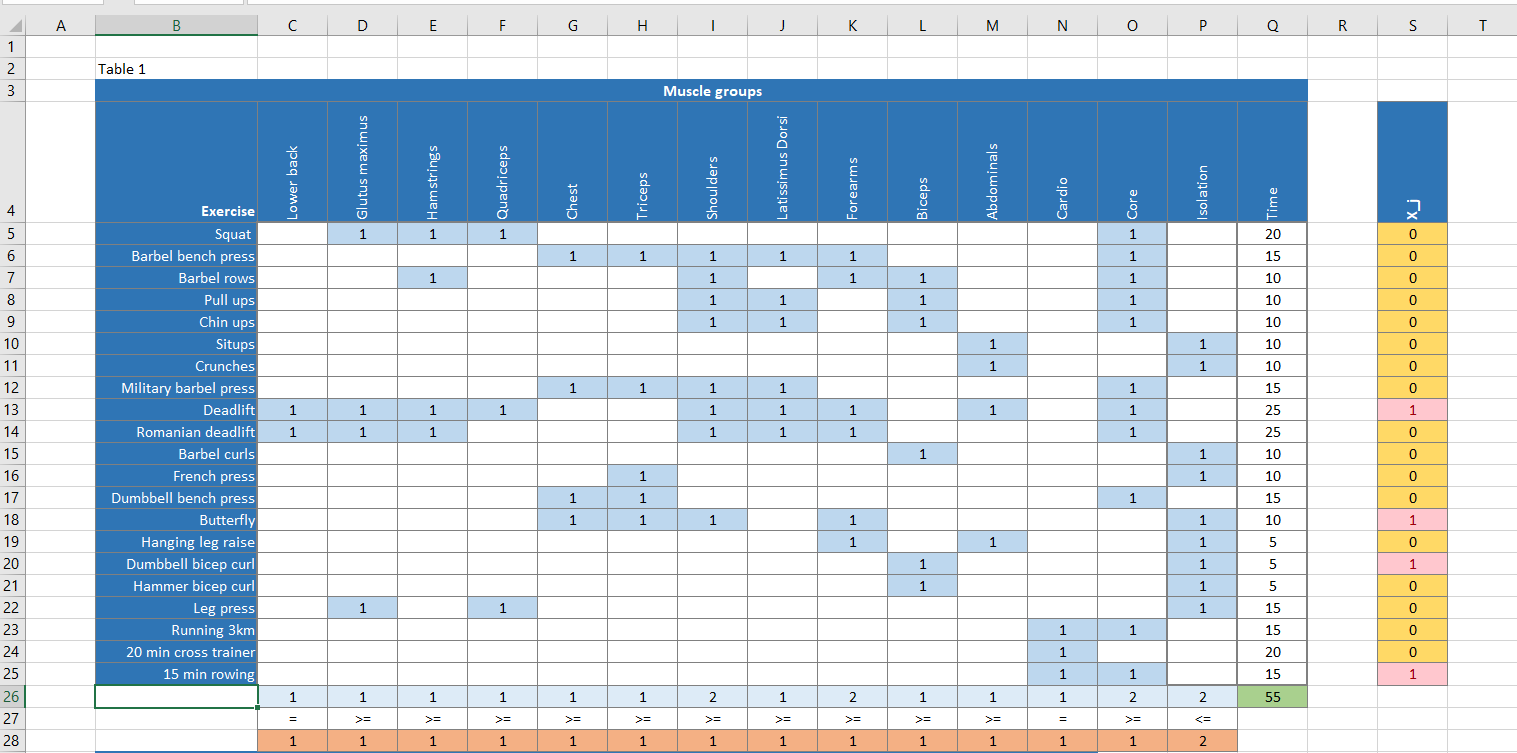
\includegraphics[width=\linewidth]{Sol2_no_formulas}}\\
                \subfloat[Screen shot of Excel with formulas after solving Task 2]{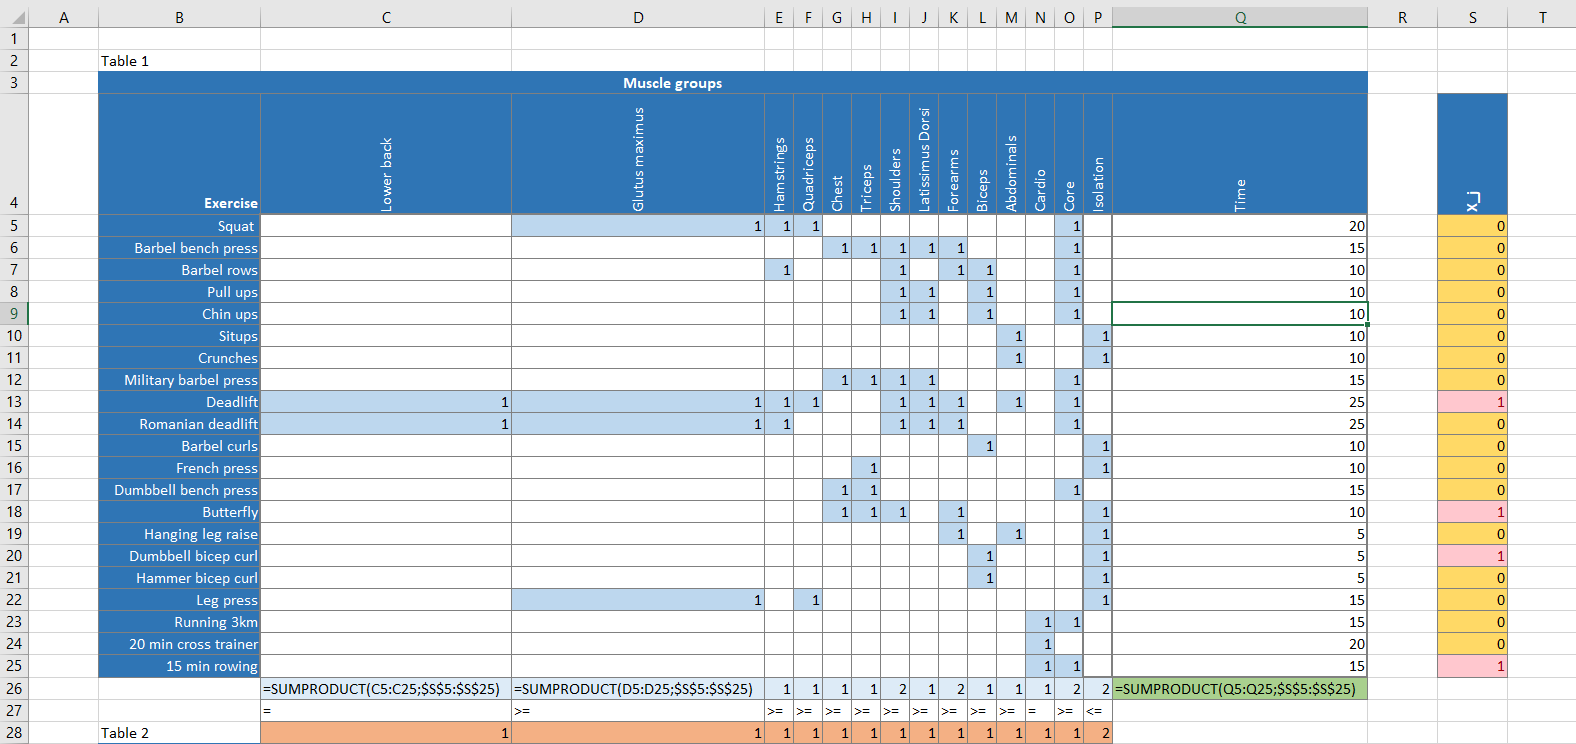
\includegraphics[width=\linewidth]{sol2_with_formulas}}
                \caption{Screen shots of Excel for Task 2}\label{fig:Task2}
        \end{figure}
    \fi
    
    \item{Task 3:} Mr. Rice does not like the program! Some of the big and important muscle groups are not targeted as he would have wanted it. He says that you must consider the information in Table~\ref{tab:2}. Change your program from \textbf{Task 1} to accommodate Mr. Rice's wishes. 
    
    \ifAnswer
        {\color{red!40!black}
            Change the right hand side of each of the constraints (except the cardio constraints) so that it reflects the information in Table~\ref{tab:2}. 
        }
    \fi
    
    \item{Task 4:} Solve the integer linear programming problem from \textbf{Task 3} and comment on the solution. Hint: An optimal program takes 100 minutes.
    
    \ifAnswer
        {\color{red!40!black}
            An optimal set of exercises is now: Squat, Barbel bench press, Pull ups, Deadlift, French press, Leg press, and 15 min rowing. The program takes 100 minus ( 1 hour and 40 minutes). See Figure~\ref{fig:Task4} for Excel details.
            
            \begin{figure}[htbp]
                \centering
                \subfloat[Screen shot of Excel without formulas after solving Task 4]{%
                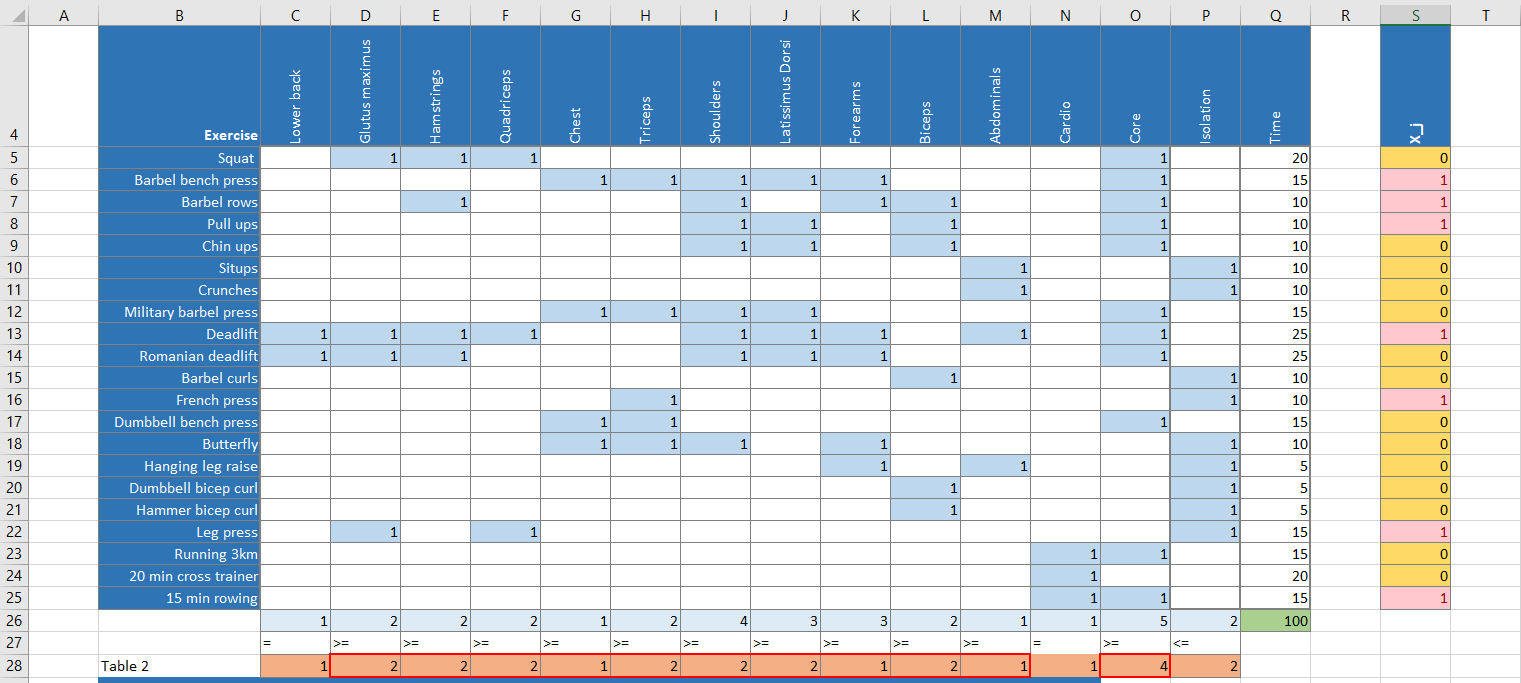
\includegraphics[width=\linewidth]{Sol4_no_formulas}}\\
                \subfloat[Screen shot of Excel with formulas after solving Task 4]{%
                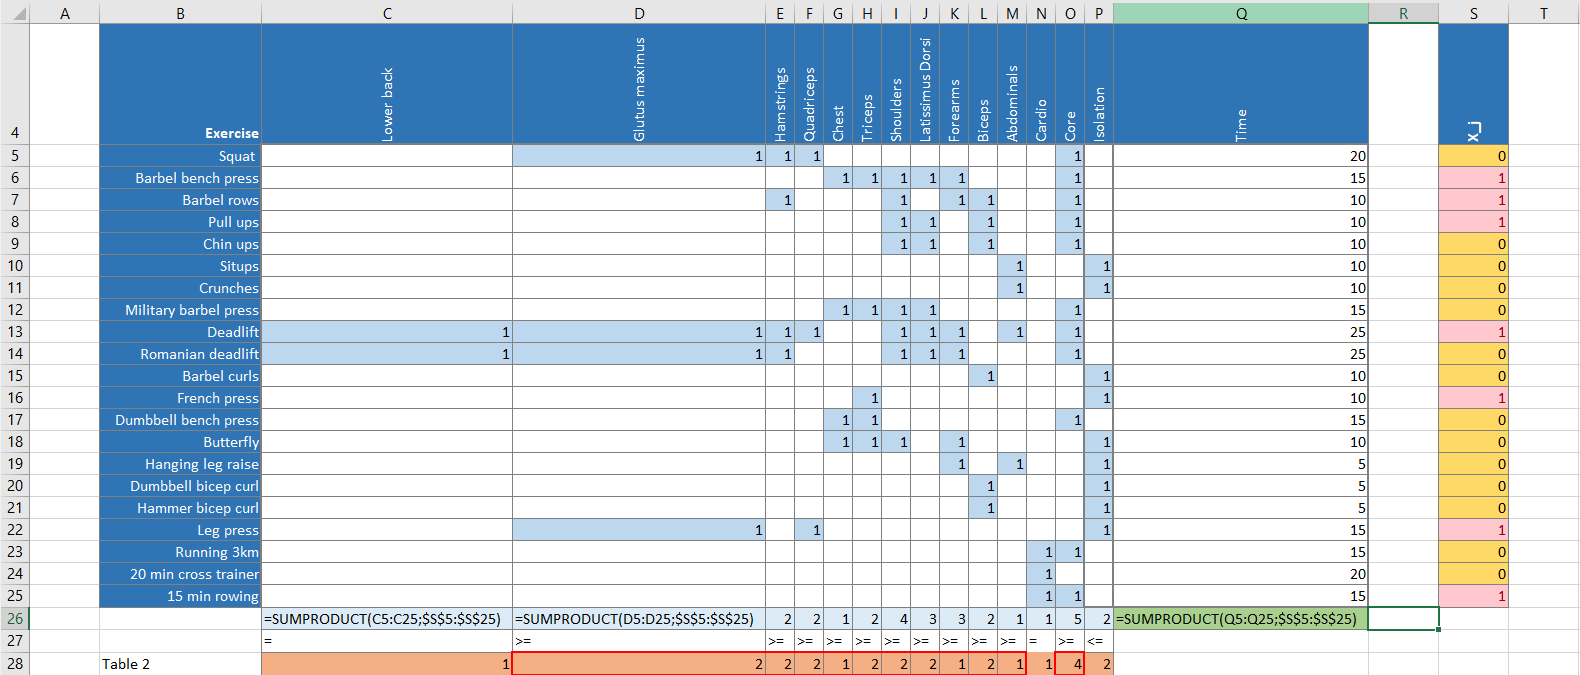
\includegraphics[width=\linewidth]{Sol4_with_formulas}}
                \caption{Screen shots of Excel for Task 4}\label{fig:Task4}
            \end{figure}
        }
    \fi
    
    \item{Task 5:} Do alternative optimal solutions to the planning problem exist? That is, can you find a different mix of exercises meeting Mr. Rice's requirements which still takes 100 minutes? Hint: If a different mix of exercises should be achieved, at least one of the exercises not chosen in \textbf{Task 4} needs to be chosen.
    
    \ifAnswer
        {\color{red!40!black}
            The answer is yes, there are several optimal solutions. To see this, add the constraint:
            \begin{align}
                &x_{\textup{Barbell rows}} + x_{\textup{Chin ups}}+ x_{\textup{Situps}}+x_{\textup{Crunches}}+ x_{\textup{Military barbel press}}\\
                &+ x_{\textup{Romanian deadlift}}
                + x_{\textup{Barbel curls}} + x_{\textup{Dumbbell bench press}} + x_{\textup{Butterfly}}\\
                &+x_{\textup{Hanging leg raise}}+ x_{\textup{Hammer bicep curl}}+x_{\textup{Leg press}} + x_{\textup{20 min cross trainer}} + x_{\textup{15 min rowing}} \geq 1
            \end{align}
            and solve the resulting problem. This leads to a solution which takes 100 minutes (so it is an alternative optimal solution). The solution consists of Squat, Barbel bench press, Chin ups, Deadlift, Frebch press, Dumbbell bicep curls, and 15 min Rowing. For Excel details see Figure~\ref{fig:Task5}.
            \begin{figure}[htbp]
                \centering
                \subfloat[Screen shot of Excel without formulas after solving Task 5]{%
                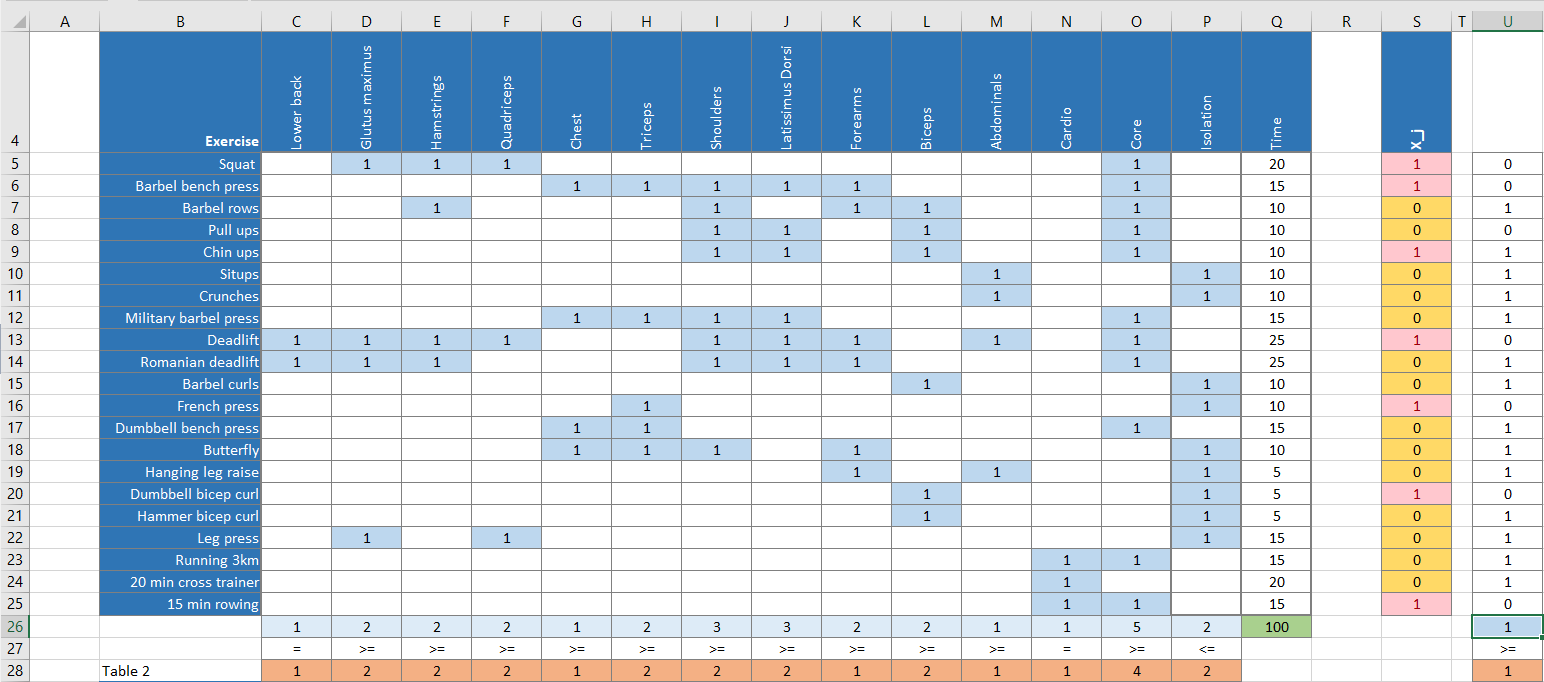
\includegraphics[width=\linewidth]{Sol5_no_formulas}}\\
                \subfloat[Screen shot of Excel with formulas after solving Task 5]{%
                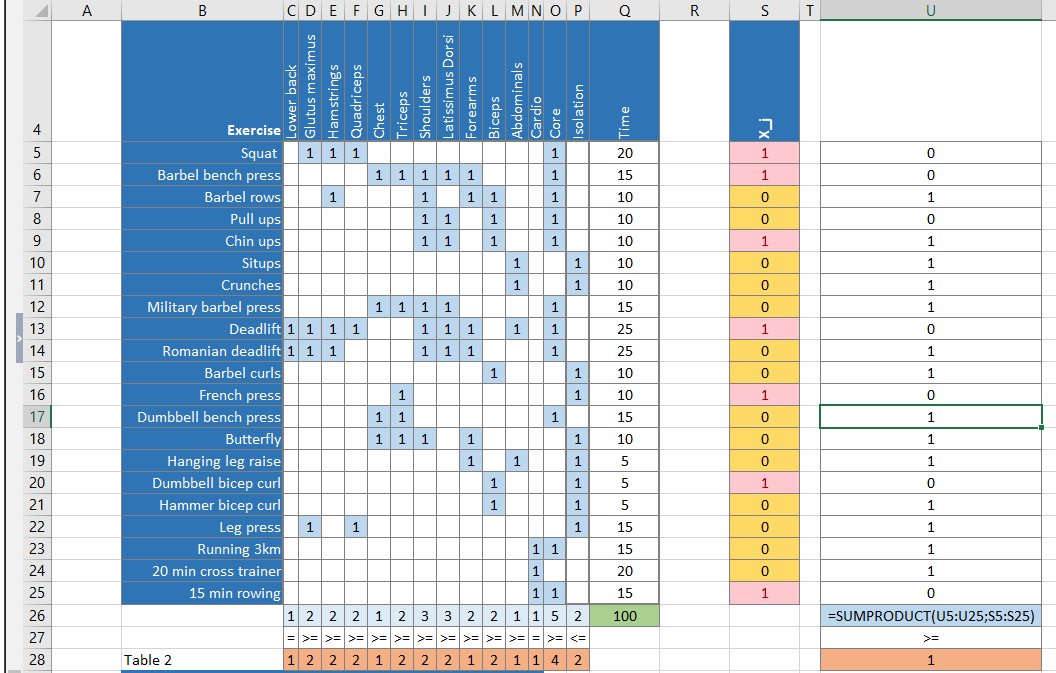
\includegraphics[width=\linewidth]{Sol5_with_formulas}}
                \caption{Screen shots of Excel for Task 5}\label{fig:Task5}
            \end{figure}
        }
    \fi
\end{description}


\ifAnswer
    \begin{figure}[htbp]
        \centering
        \subfloat[Solver window Task 2]{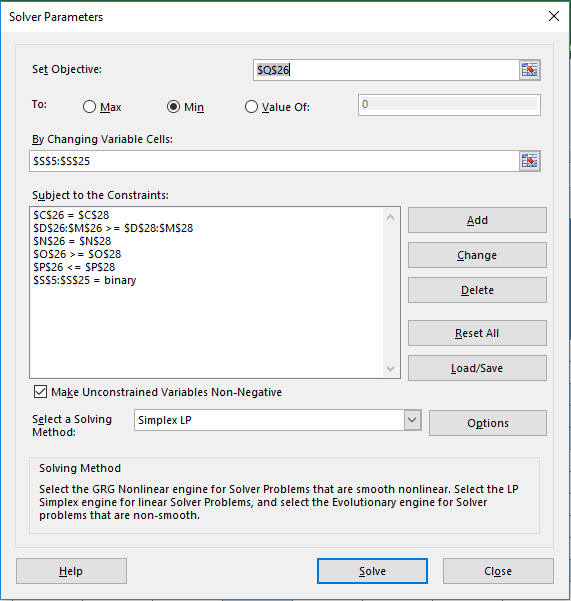
\includegraphics[width=0.45\linewidth]{Sol2_solver}}
        \subfloat[Solver window Task 4]{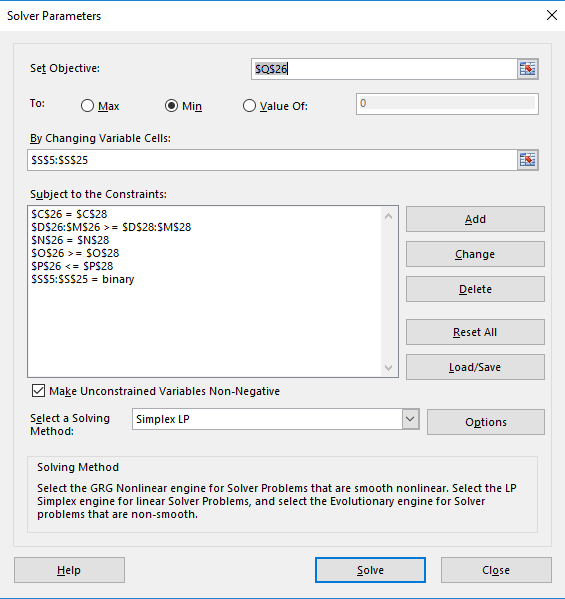
\includegraphics[width=0.45\linewidth]{Sol4_solver}}\\
        \subfloat[Solver window Task 5]{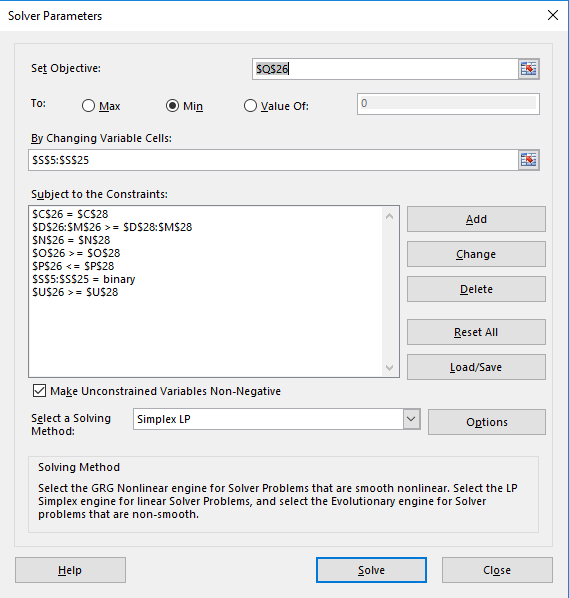
\includegraphics[width=0.45\linewidth]{Sol5_solver}}
        \caption{Solver settings for Tasks 2,4, and 5.}
    \end{figure}
\fi


\begin{landscape}
%\pagestyle{empty}
\begin{table}\small
	\centering
	\caption{Overview of the muscle groups trained by different exercises. The ``isolation'' indicates whether the exercise is an exercise which isolates a few muscle groups. The time it takes to perform an exercise is given in minutes.}\label{tab:1}
	\resizebox{\linewidth}{!}{
	\begin{tabular}{l c c c c c c c c c c c c c |c| c}
		\toprule
				& \multicolumn{13}{c}{Muscle groups}&\multicolumn{2}{c}{}\\\cmidrule{2-14}
		Exercise	& \rotatebox[origin=c]{\myAngle}{Lower back (1)}	& \rotatebox[origin=c]{\myAngle}{Glutus maximus (2)}	& \rotatebox[origin=c]{\myAngle}{Hamstrings (3)}	& \rotatebox[origin=c]{\myAngle}{Quadriceps (4)}	& \rotatebox[origin=c]{\myAngle}{Chest (5)}	& \rotatebox[origin=c]{\myAngle}{Triceps (6)}	& \rotatebox[origin=c]{\myAngle}{Shoulders (7)}	& \rotatebox[origin=c]{\myAngle}{Latissimus dorsi (8)}	& \rotatebox[origin=c]{\myAngle}{Forearms (9)}	& \rotatebox[origin=c]{\myAngle}{Biceps (10)}	& \rotatebox[origin=c]{\myAngle}{Abdominals (11)}	& \rotatebox[origin=c]{\myAngle}{Cardio (12)}	& \rotatebox[origin=c]{\myAngle}{Core (13)}	& \rotatebox[origin=c]{\myAngle}{Isolation} & \rotatebox[origin=c]{\myAngle}{Time}\\\midrule
		
		\multicolumn{1}{l|}{Squat (1)} 				&&\colorCell&\colorCell&\colorCell&&&&&&&&&\colorCell& & 20\\
		\multicolumn{1}{l|}{Barbel bench press (2)}	&&&&&\colorCell&\colorCell&\colorCell&\colorCell&\colorCell&&&&\colorCell& & 15\\
		\multicolumn{1}{l|}{Barbel rows (3)}		&&&\colorCell&&&&\colorCell&&\colorCell&\colorCell&&&\colorCell& & 10\\
		\multicolumn{1}{l|}{Pull ups (4)}			&&&&&&&\colorCell&\colorCell&&\colorCell&&&\colorCell& & 10\\
		\multicolumn{1}{l|}{Chin ups (5)}			&&&&&&&\colorCell&\colorCell&&\colorCell&&&\colorCell& & 10 \\
		\multicolumn{1}{l|}{Situps (6)}				&&&&&&&&&&&\colorCell&&&\colorCell & 10\\
		\multicolumn{1}{l|}{Crunches (7)}			&&&&&&&&&&&\colorCell&&&\colorCell & 10\\
		\multicolumn{1}{l|}{Military barbel press (8)}&&&&&\colorCell&\colorCell&\colorCell&\colorCell&&&&&\colorCell& & 15\\
		\multicolumn{1}{l|}{Deadlift (9)}         &\colorCell&\colorCell&\colorCell&\colorCell&&&\colorCell&\colorCell&\colorCell&&\colorCell&&\colorCell& & 25\\
		\multicolumn{1}{l|}{Romanian deadlift (10)}	&\colorCell&\colorCell&\colorCell&&&&\colorCell&\colorCell&\colorCell&&&&\colorCell& & 25\\
		\multicolumn{1}{l|}{Barbel curls (11)}		&&&&&&&&&&\colorCell&&&&\colorCell & 10\\
		\multicolumn{1}{l|}{French press (12)}		&&&&&&\colorCell&&&&&&&&\colorCell & 10\\
		\multicolumn{1}{l|}{Dumbbell bench press (13)}&&&&&\colorCell&\colorCell&&&&&&&\colorCell& & 15\\
		\multicolumn{1}{l|}{Butterfly (14)}			&&&&&\colorCell&\colorCell&\colorCell&&\colorCell&&&&&\colorCell & 10\\
		\multicolumn{1}{l|}{Hanging leg raise (15)}	&&&&&&&&&\colorCell&&\colorCell&&&\colorCell & 5\\
		\multicolumn{1}{l|}{Dumbbell bicep curl (16)}&&&&&&&&&&\colorCell&&&&\colorCell & 5\\
		\multicolumn{1}{l|}{Hammer bicep curl (17)}	&&&&&&&&&&\colorCell&&&&\colorCell & 5\\
		\multicolumn{1}{l|}{Leg press (18)}			&&\colorCell&&\colorCell&&&&&&&&&&\colorCell & 15\\
		\multicolumn{1}{l|}{Running 3km (19)}		&&&&&&&&&&&&\colorCell&\colorCell& & 15\\
		\multicolumn{1}{l|}{20 min cross trainer (20)}&&&&&&&&&&&&\colorCell&& & 20\\
		\multicolumn{1}{l|}{15 min rowing (21)}		&&&&&&&&&&&&\colorCell&\colorCell& & 15\\
		\bottomrule
	\end{tabular}}
\end{table}
\end{landscape}

\begin{landscape}
%\pagestyle{empty}
	\begin{table}\small
	\centering
	\caption{Overview of Mr. Rice's additional requirements to the program. The entries denote the minimum number of exercises in the program targeting the corresponding muscle group.}\label{tab:2}
	\resizebox{\linewidth}{!}{
	\begin{tabular}{l c c c c c c c c c c c  c }
		\toprule
				& \multicolumn{12}{c}{Muscle groups}\\\cmidrule{2-13}
		Exercise	& \rotatebox[origin=c]{\myAngle}{Lower back (1)}	& \rotatebox[origin=c]{\myAngle}{Glutus maximus (2)}	& \rotatebox[origin=c]{\myAngle}{Hamstrings (3)}	& \rotatebox[origin=c]{\myAngle}{Quadriceps (4)}	& \rotatebox[origin=c]{\myAngle}{Chest (5)}	& \rotatebox[origin=c]{\myAngle}{Triceps (6)}	& \rotatebox[origin=c]{\myAngle}{Shoulders (7)}	& \rotatebox[origin=c]{\myAngle}{Latissimus dorsi (8)}	& \rotatebox[origin=c]{\myAngle}{Forearms (9)}	& \rotatebox[origin=c]{\myAngle}{Biceps (10)}	& \rotatebox[origin=c]{\myAngle}{Abdominals (11)}	& \rotatebox[origin=c]{\myAngle}{Core (13)}\\\midrule
		Number of exercises & 1&	2&	2&	2&	1&	2&	2&	2&	1&	2&	1&	4\\\bottomrule
	\end{tabular}}
\end{table}
\end{landscape}

\end{document}